%%%%%%%%%%%%%%%%%%%%%%%%%%%%%%%%%%%%%%%%%%%%%%%%%%%%%%%%%%%%%%%%%%%%%%%%%%%%%%%%
% Job Apply Agent — proposed architecture (multi-source fetch + classify +
% multi-select job-type dropdown). UML class diagram + data-flow diagram.
% Compile: pdflatex architecture.tex   (needs only the tikz package)
%%%%%%%%%%%%%%%%%%%%%%%%%%%%%%%%%%%%%%%%%%%%%%%%%%%%%%%%%%%%%%%%%%%%%%%%%%%%%%%%
\documentclass[11pt]{article}
\usepackage[T1]{fontenc}
\usepackage[a4paper,landscape,margin=1cm]{geometry}
\usepackage{tikz}
\usepackage{xcolor}
\usetikzlibrary{shapes.multipart, shapes.geometric, arrows.meta, positioning, fit, backgrounds, calc}

\tikzset{
  class/.style={
    rectangle split, rectangle split parts=2, rounded corners=1.5pt,
    draw=black!55, fill=blue!5, line width=0.4pt,
    text width=34mm, align=left, font=\scriptsize, inner sep=3pt},
  iface/.style ={class, fill=green!7},
  entity/.style={class, fill=orange!8},
  ui/.style    ={class, fill=violet!8},
  store/.style ={class, fill=cyan!7},
  realize/.style={-{Triangle[open]}, dashed, draw=black!55},   % interface realization
  assoc/.style  ={-{Stealth}, draw=black!70},                  % association / uses
  depend/.style ={-{Stealth}, dashed, draw=black!55},          % dependency
  note/.style   ={rectangle, rounded corners=1pt, draw=black!40,
                  fill=yellow!18, font=\scriptsize\itshape, text width=44mm,
                  align=left, inner sep=3pt},
  flow/.style   ={rectangle, rounded corners=3pt, draw=black!60, line width=0.5pt,
                  fill=blue!5, align=center, font=\small, minimum height=9mm,
                  inner sep=4pt, text width=34mm},
  decision/.style={diamond, aspect=2, draw=black!60, fill=orange!12,
                  align=center, font=\scriptsize, inner sep=1pt},
  farrow/.style   ={-{Stealth}, draw=black!75, line width=0.6pt, font=\scriptsize},
}

\begin{document}
\pagestyle{empty}

%======================================================================
% Figure 1 — Class diagram
%======================================================================
\begin{center}
{\Large\bfseries Job Apply Agent — Class Diagram (proposed multi-source + classification)}\\[1mm]
{\footnotesize Green = interface \quad Blue = service \quad Orange = entity \quad Cyan = persistence \quad Violet = UI}
\end{center}
\vspace{2mm}

\noindent\resizebox{\textwidth}{!}{%
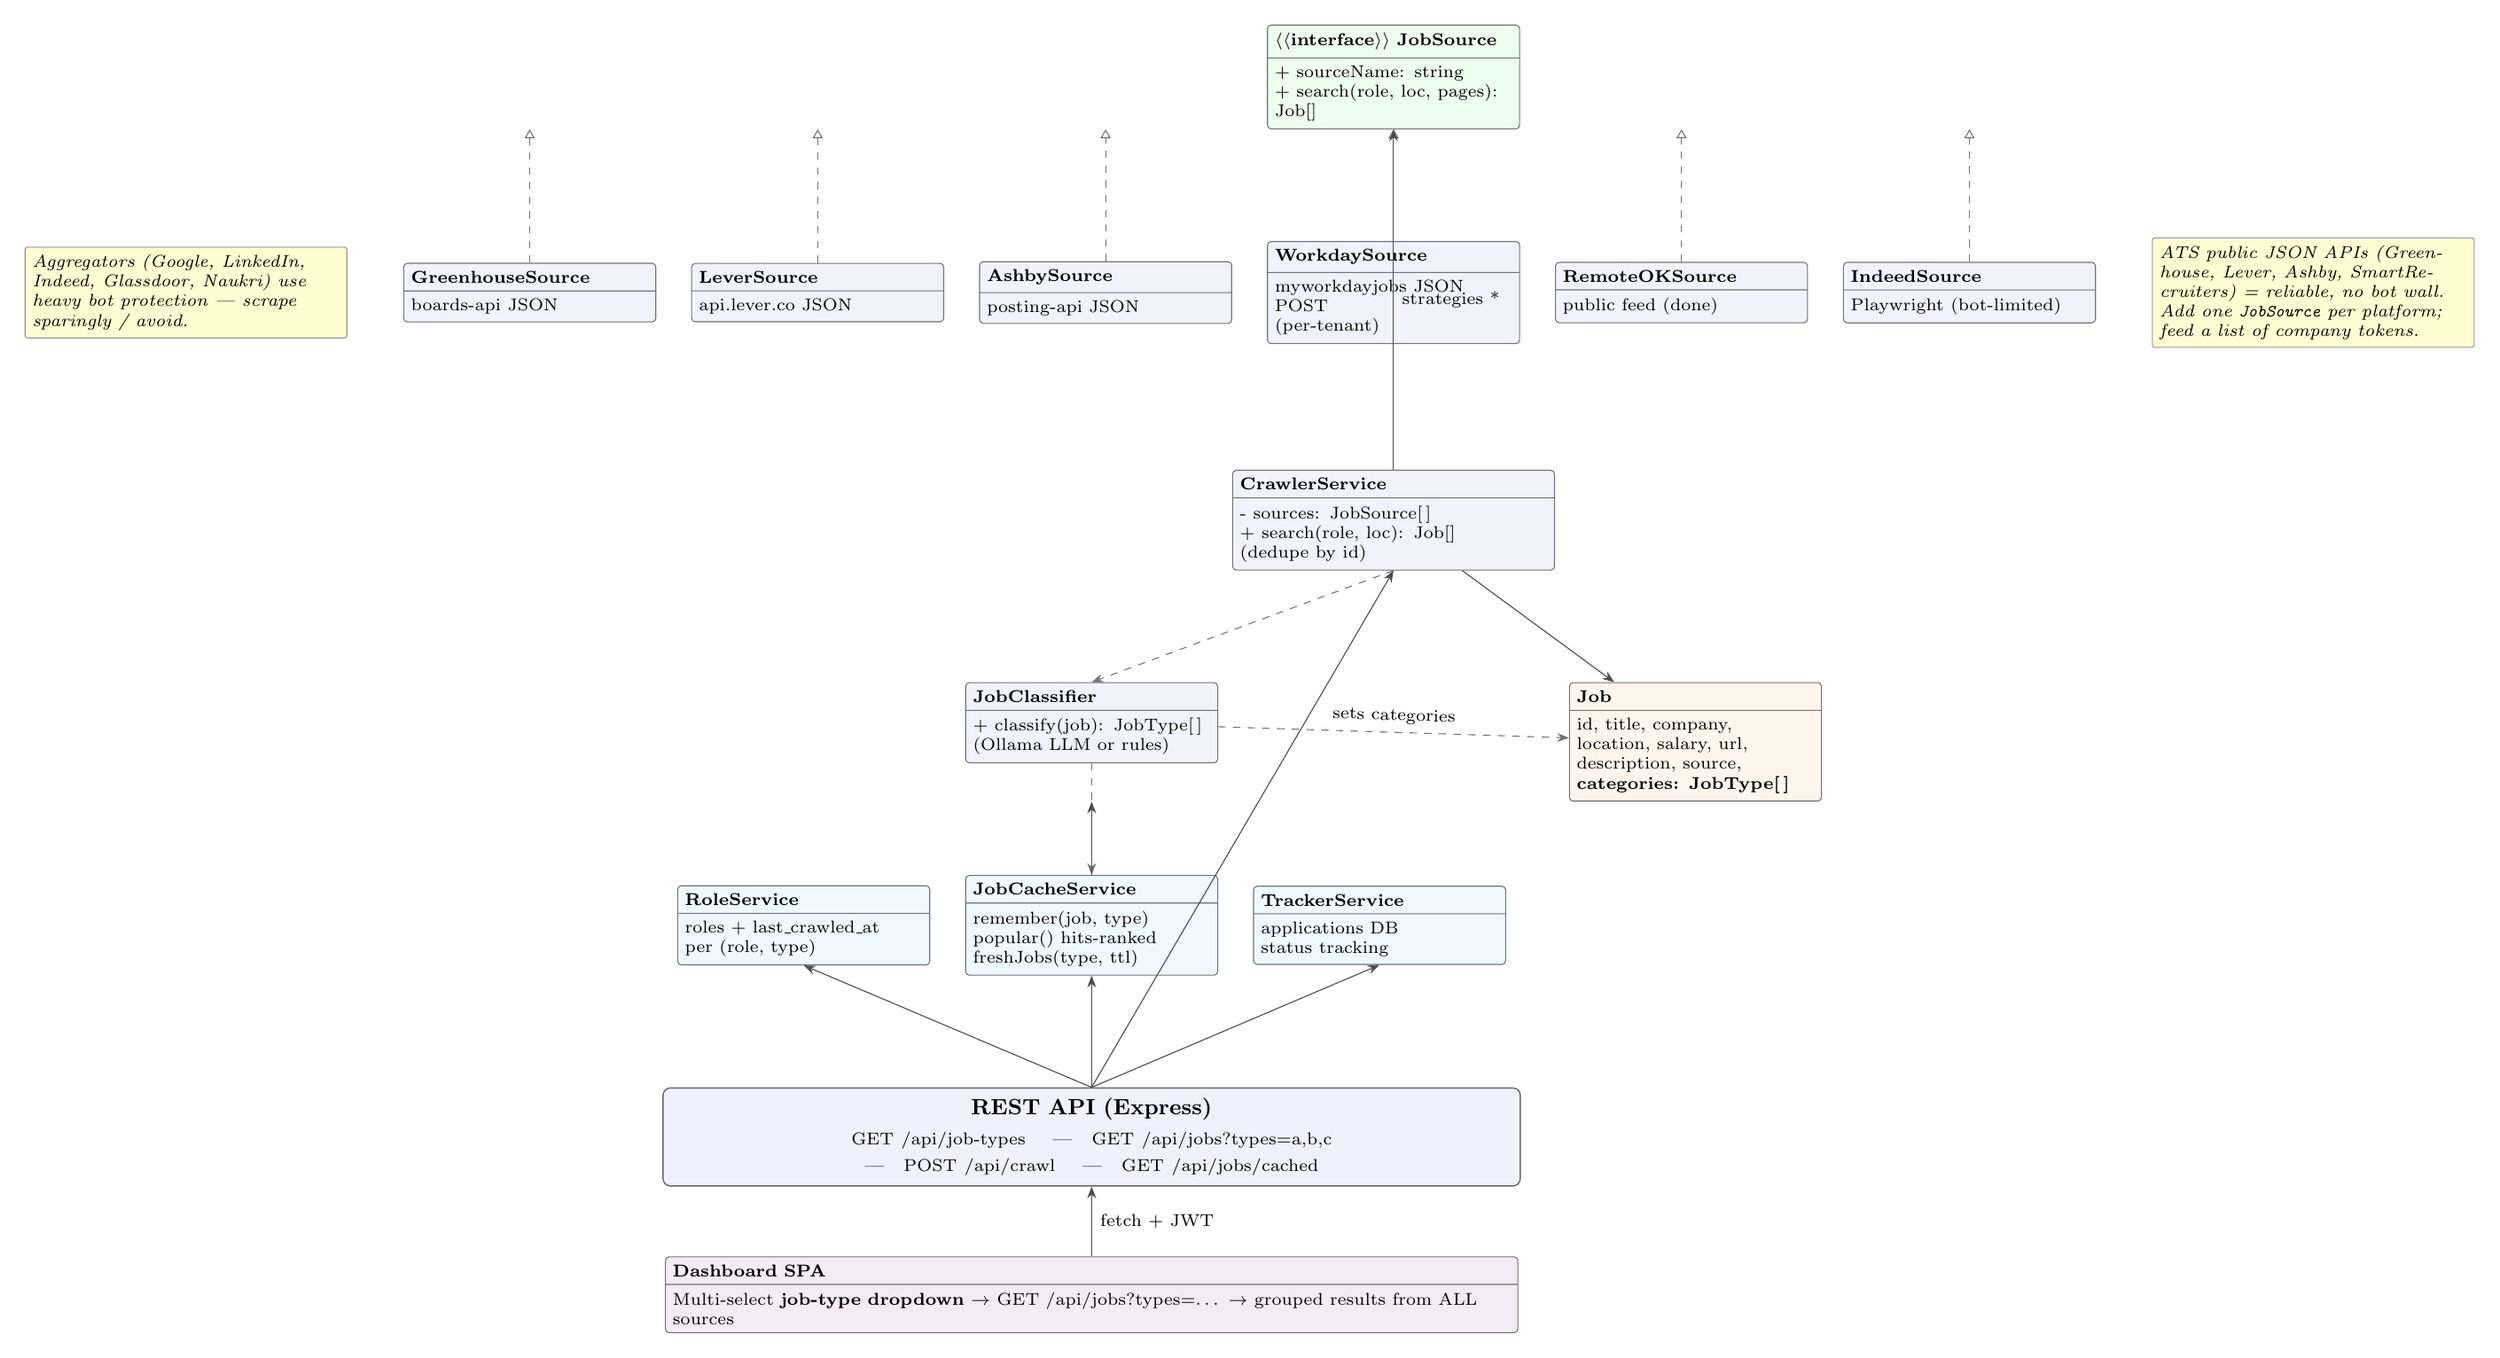
\begin{tikzpicture}[node distance=6mm and 5mm]

% ---- interface ----
\node[iface] (js) {%
  \textbf{$\langle\langle$interface$\rangle\rangle$ JobSource}
  \nodepart{second}+ sourceName: string\\+ search(role, loc, pages): Job[]};

% ---- concrete sources (Strategy implementations) ----
\node[class, below=16mm of js] (workday)   {\textbf{WorkdaySource}\nodepart{second}myworkdayjobs JSON POST\\(per-tenant)};
\node[class, left=5mm of workday]  (ashby)  {\textbf{AshbySource}\nodepart{second}posting-api JSON};
\node[class, left=5mm of ashby]    (lever)  {\textbf{LeverSource}\nodepart{second}api.lever.co JSON};
\node[class, left=5mm of lever]    (green)  {\textbf{GreenhouseSource}\nodepart{second}boards-api JSON};
\node[class, right=5mm of workday] (remote) {\textbf{RemoteOKSource}\nodepart{second}public feed (done)};
\node[class, right=5mm of remote]  (indeed) {\textbf{IndeedSource}\nodepart{second}Playwright (bot-limited)};

\foreach \s in {green,lever,ashby,workday,remote,indeed}
  \draw[realize] (\s.north) -- (\s.north |- js.south);

% ---- aggregation / orchestration ----
\node[class, below=18mm of workday, text width=44mm] (crawler) {%
  \textbf{CrawlerService}
  \nodepart{second}- sources: JobSource[\,]\\+ search(role, loc): Job[]\\(dedupe by id)};
\draw[assoc] (crawler) -- node[right,font=\scriptsize] {strategies *} (js);

% ---- classifier + entity ----
\node[class, below left=16mm and 2mm of crawler] (classifier) {%
  \textbf{JobClassifier}
  \nodepart{second}+ classify(job): JobType[\,]\\(Ollama LLM or rules)};
\node[entity, below right=16mm and 2mm of crawler] (job) {%
  \textbf{Job}
  \nodepart{second}id, title, company,\\location, salary, url,\\description, source,\\\textbf{categories: JobType[\,]}};
\draw[assoc]  (crawler) -- (job);
\draw[depend] (classifier) -- node[above,font=\scriptsize,sloped] {sets categories} (job);
\draw[depend] (crawler.south) -- (classifier.north);

% ---- persistence ----
\node[store, below=16mm of classifier] (cache) {%
  \textbf{JobCacheService}
  \nodepart{second}remember(job, type)\\popular() hits-ranked\\freshJobs(type, ttl)};
\node[store, left=5mm of cache] (role) {%
  \textbf{RoleService}
  \nodepart{second}roles + last\_crawled\_at\\per (role, type)};
\node[store, right=5mm of cache] (tracker) {%
  \textbf{TrackerService}
  \nodepart{second}applications DB\\status tracking};
\draw[depend] (classifier) -- (cache);
\draw[assoc]  (cache) -- (job.south -| cache.north);

% ---- API ----
\node[flow, below=16mm of cache, text width=120mm, fill=blue!6] (api) {%
  \textbf{REST API (Express)} \\[0.5mm]
  \scriptsize GET /api/job-types \quad|\quad GET /api/jobs?types=a,b,c \quad|\quad POST /api/crawl \quad|\quad GET /api/jobs/cached};
\foreach \s in {role,cache,tracker,crawler}
  \draw[assoc] (api.north) -- (\s.south);

% ---- UI ----
\node[ui, below=10mm of api, text width=120mm] (ui) {%
  \textbf{Dashboard SPA} \nodepart{second}%
  Multi-select \textbf{job-type dropdown} $\rightarrow$ GET /api/jobs?types=\dots\ $\rightarrow$ grouped results from ALL sources};
\draw[assoc] (ui) -- node[right,font=\scriptsize] {fetch + JWT} (api);

% ---- notes ----
\node[note, right=8mm of indeed] (n1) {ATS public JSON APIs (Greenhouse, Lever, Ashby, SmartRecruiters) = reliable, no bot wall. Add one \texttt{JobSource} per platform; feed a list of company tokens.};
\node[note, left=8mm of green] (n2) {Aggregators (Google, LinkedIn, Indeed, Glassdoor, Naukri) use heavy bot protection — scrape sparingly / avoid.};

\end{tikzpicture}}

\newpage
%======================================================================
% Figure 2 — Data-flow
%======================================================================
\begin{center}
{\Large\bfseries Data Flow — user picks job types, sees roles from all sources}
\end{center}
\vspace{4mm}

\noindent\resizebox{\textwidth}{!}{%
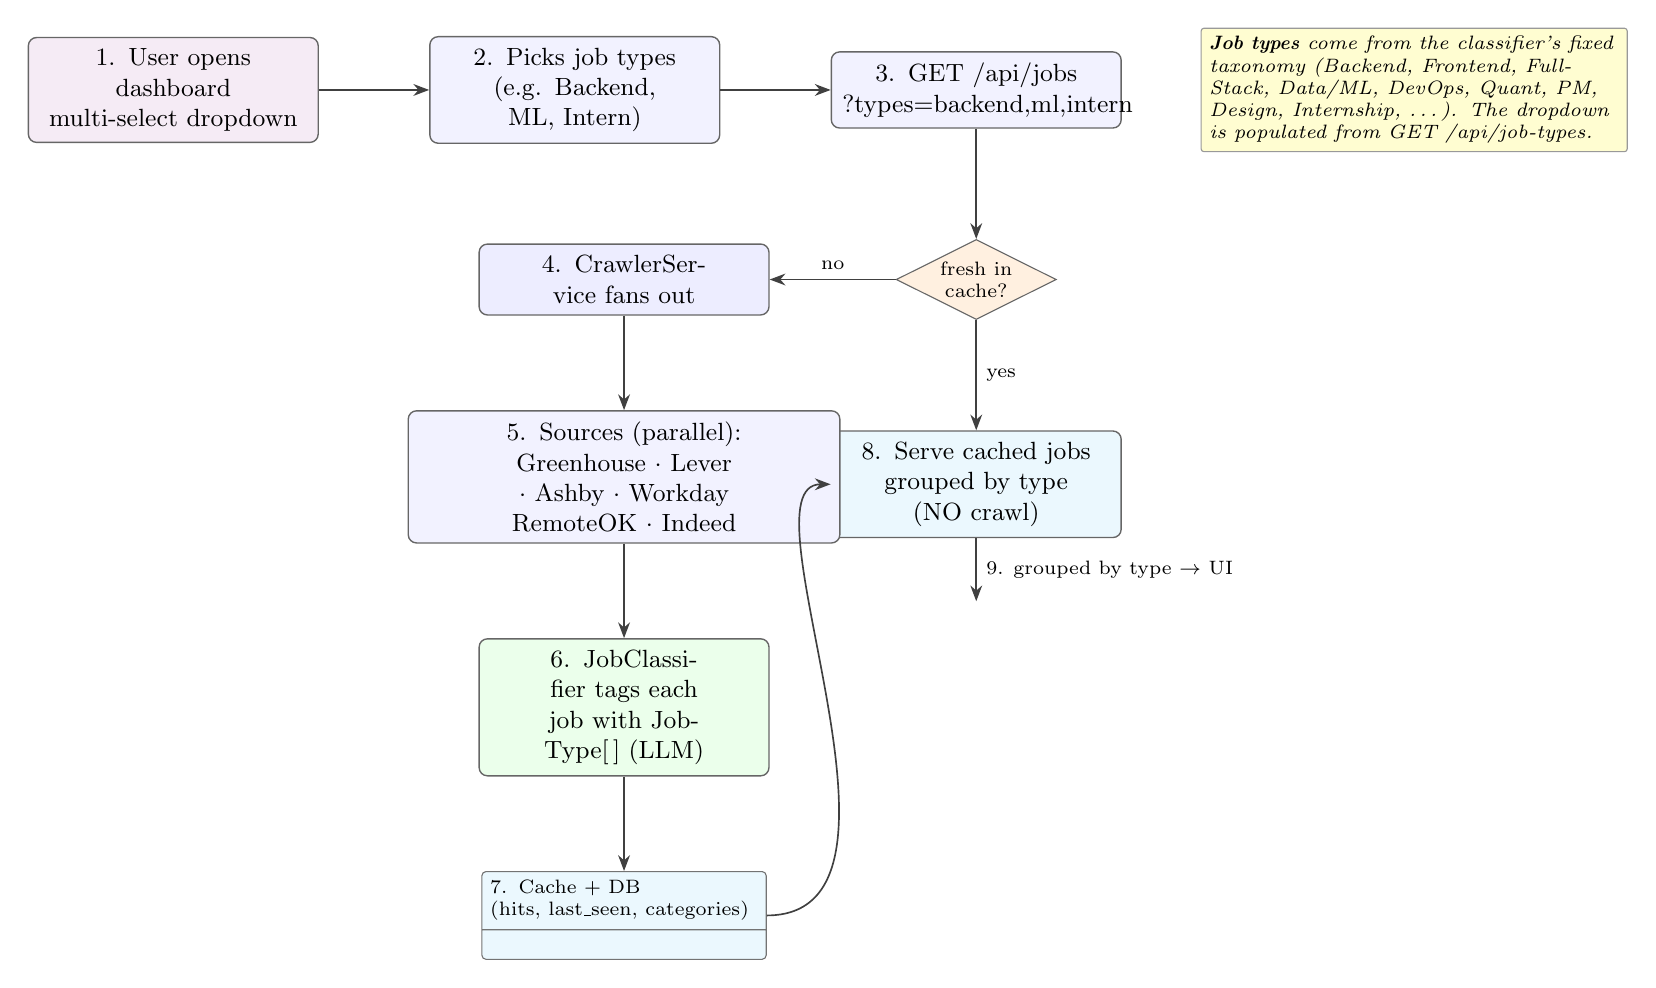
\begin{tikzpicture}[node distance=10mm]

\node[flow, fill=violet!8] (u1) {1. User opens dashboard\\multi-select dropdown};
\node[flow, right=14mm of u1] (u2) {2. Picks job types\\(e.g. Backend, ML, Intern)};
\node[flow, right=14mm of u2] (u3) {3. GET /api/jobs\\?types=backend,ml,intern};

\node[decision, below=14mm of u3] (d1) {fresh in\\cache?};
\node[flow, below=14mm of d1, fill=cyan!8] (serve) {8. Serve cached jobs\\grouped by type (NO crawl)};

\node[flow, left=16mm of d1, fill=blue!7] (crawl) {4. CrawlerService fans out};
\node[flow, below=12mm of crawl, text width=52mm] (sources) {5. Sources (parallel):\\Greenhouse $\cdot$ Lever $\cdot$ Ashby $\cdot$ Workday\\RemoteOK $\cdot$ Indeed};
\node[flow, below=12mm of sources, fill=green!8] (classify) {6. JobClassifier tags each\\job with JobType[\,] (LLM)};
\node[store, below=12mm of classify, fill=cyan!8] (persist) {7. Cache + DB\\(hits, last\_seen, categories)};

\draw[farrow] (u1) -- (u2);
\draw[farrow] (u2) -- (u3);
\draw[farrow] (u3) -- (d1);
\draw[farrow] (d1) -- node[above,font=\scriptsize]{no} (crawl);
\draw[farrow] (d1) -- node[right,font=\scriptsize]{yes} (serve);
\draw[farrow] (crawl) -- (sources);
\draw[farrow] (sources) -- (classify);
\draw[farrow] (classify) -- (persist);
\draw[farrow] (persist.east) .. controls +(right:22mm) and +(left:12mm) .. (serve.west);
\draw[farrow] (serve) -- node[right,font=\scriptsize]{9. grouped by type $\rightarrow$ UI} ($(serve.south)+(0,-8mm)$);

\node[note, right=10mm of u3, text width=52mm] {\textbf{Job types} come from the classifier's fixed taxonomy (Backend, Frontend, Full-Stack, Data/ML, DevOps, Quant, PM, Design, Internship, \dots). The dropdown is populated from GET /api/job-types.};

\end{tikzpicture}}

\end{document}
